\documentclass[tikz, border=10pt]{standalone}
\usetikzlibrary{shapes.geometric, arrows, positioning}

\begin{document}
	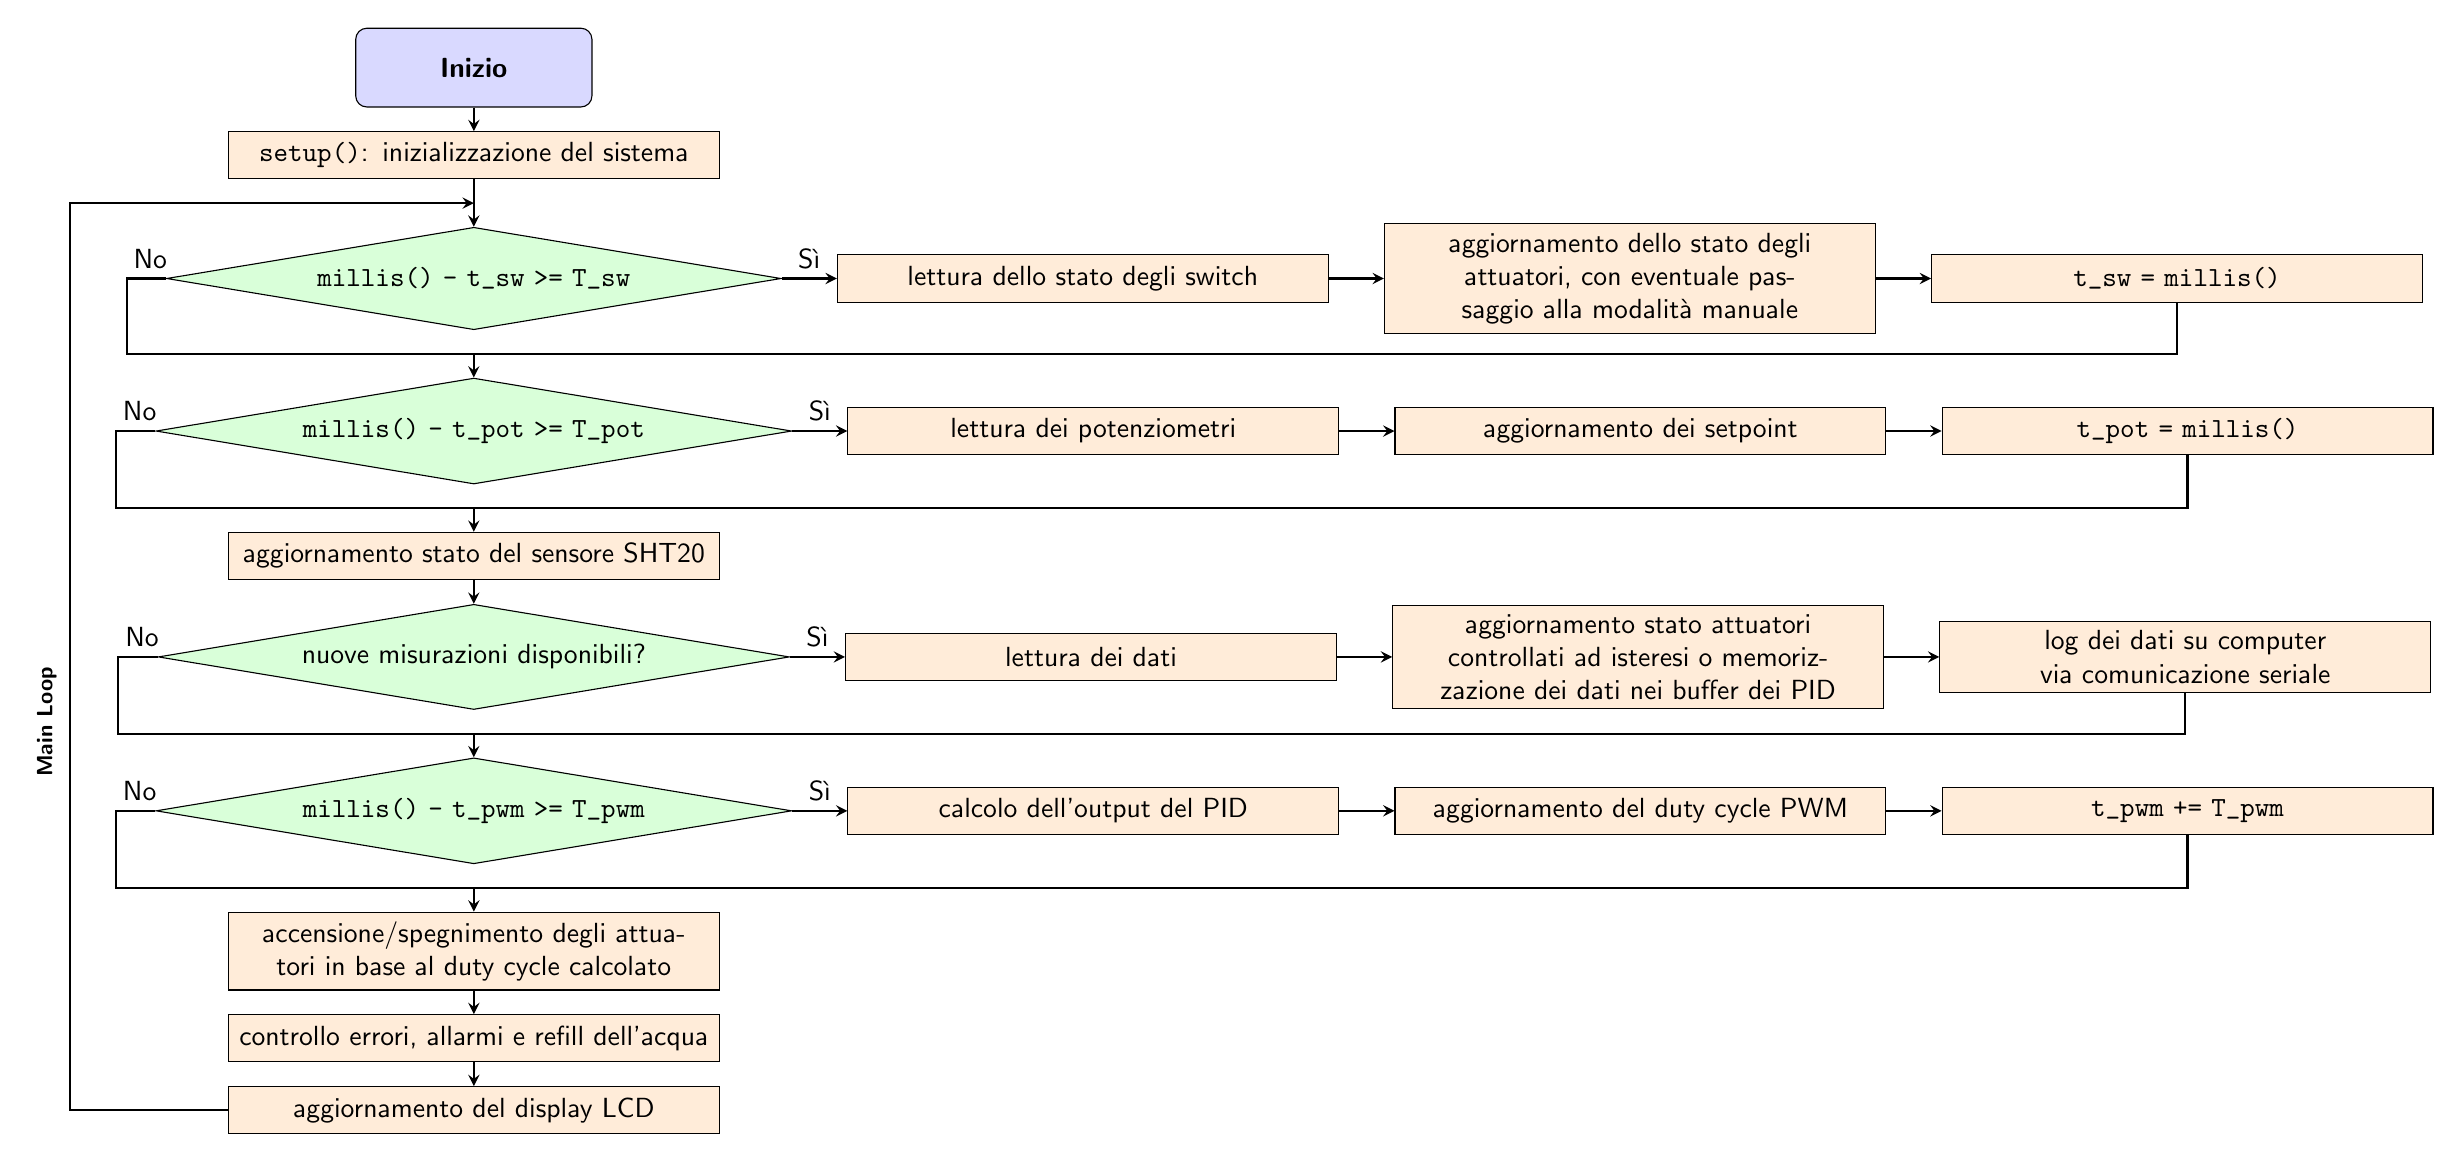
\begin{tikzpicture}[
			node distance=0.3cm and 0.7cm,
			startstop/.style={rectangle, rounded corners, minimum width=3cm, minimum height=1cm, align=center, draw=black, fill=blue!15, font=\sffamily\bfseries},
			process1/.style={rectangle, minimum width=2cm, minimum height=0.6cm, align=center, draw=black, fill=orange!15, text width=6cm, font=\sffamily},
			process2/.style={rectangle, minimum width=2cm, minimum height=0.6cm, align=center, draw=black, fill=orange!15, text width=6cm, font=\sffamily},
			decision/.style={diamond, minimum width=6cm, minimum height=1cm, align=center, draw=black, fill=green!15, aspect=6, text width=4.5cm, font=\sffamily},
			dec_label/.style={font=\sffamily, anchor=south},
			arrow/.style={thick,->,>=stealth},
			line/.style={thick}
		]

		% --- PARTE DI SETUP ---
		\node (start) [startstop] at (0,0) {Inizio};
		\node (setup) [process1, below=of start] {\verb|setup()|: inizializzazione del sistema};

		% --- PARTE DI LOOP PERIODICO ---
		% Blocco tempo
		\node (loop) [coordinate, below=of setup] {};

		% --- TASK 1: GESTIONE SWITCH ---
		\node (dec_sw) [decision, below=of loop] {\verb|millis() - t_sw >= T_sw|};
		\node (task_sw1) [process2, right=of dec_sw] {lettura dello stato degli switch};
		\node (task_sw2) [process2, right=of task_sw1] {aggiornamento dello stato degli attuatori, con eventuale passaggio alla modalità manuale};
		\node (reset_sw) [process2, right=of task_sw2] {\verb|t_sw = millis()|};
		\node (conv_sw) [coordinate, below=of dec_sw] {};

		% --- TASK 2: AGGIORNAMENTO SETPOINT ---
		\node (dec_pot) [decision, below=of conv_sw] {\verb|millis() - t_pot >= T_pot|};
		\node (task_pot1) [process2, right=of dec_pot] {lettura dei potenziometri};
		\node (task_pot2) [process2, right=of task_pot1] {aggiornamento dei setpoint};
		\node (reset_pot) [process2, right=of task_pot2] {\verb|t_pot = millis()|};
		\node (conv_pot) [coordinate, below=of dec_pot] {};

		% --- TASK 3: GESTIONE SENSORE SHT20 ---
		\node (sht_update) [process1, below=of conv_pot] {aggiornamento stato del sensore SHT20};
		\node (dec_sht) [decision, below=of sht_update] {nuove misurazioni disponibili?};
		\node (task_sht1) [process2, right=of dec_sht] {lettura dei dati};
		\node (task_sht2) [process2, right=of task_sht1] {aggiornamento stato attuatori controllati ad isteresi o memorizzazione dei dati nei buffer dei PID};
		\node (log_sht) [process2, right=of task_sht2] {log dei dati su computer via comunicazione seriale};
		\node (conv_sht) [coordinate, below=of dec_sht] {};

		% --- TASK 4: AGGIORNAMENTO PID e DUTY CYCLE ---
		\node (dec_pwm) [decision, below=of conv_sht] {\verb|millis() - t_pwm >= T_pwm|};
		\node (task_pwm1) [process2, right=of dec_pwm] {calcolo dell'output del PID};
		\node (task_pwm2) [process2, right=of task_pwm1] {aggiornamento del duty cycle PWM};
		\node (reset_pwm) [process2, right=of task_pwm2] {\verb|t_pwm += T_pwm|};
		\node (conv_pwm) [coordinate, below=of dec_pwm] {};

		% --- PARTE DI LOOP NON PERIODICO (eseguito ogni ciclo) ---
		\node (pwm_update) [process1, below=of conv_pwm] {accensione/spegnimento degli attuatori in base al duty cycle calcolato};
		\node (alarms) [process1, below=of pwm_update] {controllo errori, allarmi e refill dell'acqua};
		\node (lcd) [process1, below=of alarms] {aggiornamento del display LCD};

		% --- COLLEGAMENTI ---
		% Setup a Loop
		\draw [arrow] (start) -- (setup);
		\draw [line] (setup) -- (loop);

		% Loop principale
		\draw [arrow] (loop) -- (dec_sw);

		% Task Switch
		\draw [arrow] (dec_sw) -- node[dec_label] {Sì} (task_sw1);
		\draw [arrow] (task_sw1) -- (task_sw2);
		\draw [arrow] (task_sw2) -- (reset_sw);
		\draw [line] (dec_sw.west) -| node[dec_label, xshift=0.3cm] {No} ++(-0.5,0) |- (conv_sw);
		\draw [line] (reset_sw) |- (conv_sw);
		\draw [arrow] (conv_sw) -- (dec_pot);

		% Task Potenziometri
		\draw [arrow] (dec_pot) -- node[dec_label] {Sì} (task_pot1);
		\draw [arrow] (task_pot1) -- (task_pot2);
		\draw [arrow] (task_pot2) -- (reset_pot);
		\draw [line] (dec_pot.west) -| node[dec_label, xshift=0.3cm] {No} ++(-0.5,0) |- (conv_pot);
		\draw [line] (reset_pot) |- (conv_pot);
		\draw [arrow] (conv_pot) -- (sht_update);

		% Task SHT20
		\draw [arrow] (sht_update) -- (dec_sht);
		\draw [arrow] (dec_sht) -- node[dec_label] {Sì} (task_sht1);
		\draw [arrow] (task_sht1) -- (task_sht2);
		\draw [arrow] (task_sht2) -- (log_sht);
		\draw [line] (dec_sht.west) -| node[dec_label, xshift=0.3cm] {No} ++(-0.5,0) |- (conv_sht);
		\draw [line] (log_sht) |- (conv_sht);
		\draw [arrow] (conv_sht) -- (dec_pwm);

		% Task PWM
		\draw [arrow] (dec_pwm) -- node[dec_label] {Sì} (task_pwm1);
		\draw [arrow] (task_pwm1) -- (task_pwm2);
		\draw [arrow] (task_pwm2) -- (reset_pwm);
		\draw [line] (dec_pwm.west) -| node[dec_label, xshift=0.3cm] {No} ++(-0.5,0) |- (conv_pwm);
		\draw [line] (reset_pwm) |- (conv_pwm);
		\draw [arrow] (conv_pwm) -- (pwm_update);

		% Blocchi non periodici
		\draw [arrow] (pwm_update) -- (alarms);
		\draw [arrow] (alarms) -- (lcd);

		% Ritorno del Loop
		\draw [arrow] (lcd.west) -| ++(-2,0) |- (loop.west) node[near start, left, xshift=-0.3cm,rotate=90, font=\sffamily\footnotesize] {\textbf{Main Loop}};
	\end{tikzpicture}
\end{document}
